\documentclass[a4paper]{article}
%\usepackage{inputenc}
\usepackage{csquotes}
\usepackage[margin=1.5cm]{geometry} % Change the margins
\usepackage[utf8]{inputenc} % - Defines what coding LaTeX uses. Use this one.
\usepackage[english]{babel}
\usepackage[T1]{fontenc}
\usepackage{graphicx} % - Package for including images in the document.
\usepackage{amsmath}
\usepackage{amssymb}
\usepackage{mathtools}
\usepackage{listings}
\usepackage{textgreek}
\usepackage{caption} % Correct spacing for captions
\usepackage{siunitx} % Package for handling numbers (ex \num{1e6}), units (ex \SI{15,3}{Nm}) and intervals (ex \SIrange{10}{20}{\celcius}) correctly
\sisetup{output-decimal-marker={,},range-phrase=--,range-units=single,exponent-product=\cdot} % If you write in English, remove output-marker...
\graphicspath{ {Images/} } % - Path to where the images are located on your computer. In this case I have a folder (look to the left) "Images" where the images are gathered.
\usepackage{hyperref} % - Package for including hyperlinks in the document.
\usepackage[style=apa,backend=biber]{biblatex} % APA-referenser
\usepackage{mhchem}
\DeclareLanguageMapping{swedish}{swedish-apa}  % APA-referenser
 % - Package for the bibliography ("referenser").
\addbibresource{references.bib} % - From where, i.e. which file, the references are taken. The bibliography file is called name.bib; see left column.

\title{Lab 3}

\author{
Author \\
{Klas Mannberg,   klaman-8@student.ltu.se
} \\ \\

\includegraphics[width=0.2\textwidth]{ltu_swe.jpg}}
\date{29 May 2020}

\begin{document}

\maketitle

\section{Exercises}
\subsection{Exercise 1}
Solved with the following two code blocks: \\
\textbf{x(t):}
\begin{lstlisting}
function x = x(t)
    x = (3/2+3/10*sin(2*pi*t)+sin((2*pi)/3*t)-sin((2*pi)/10*t)).*sinc(t);
\end{lstlisting}
\textbf{And for the plot:}
\begin{lstlisting}
function Ex1 = Ex1()
    t = -5:0.1:5;
    plot(t,x(t));
    xlabel('t');
    ylabel('x(t)');
\end{lstlisting}
See figure \ref{fig:1} for the result.
\begin{figure}
    \centering
    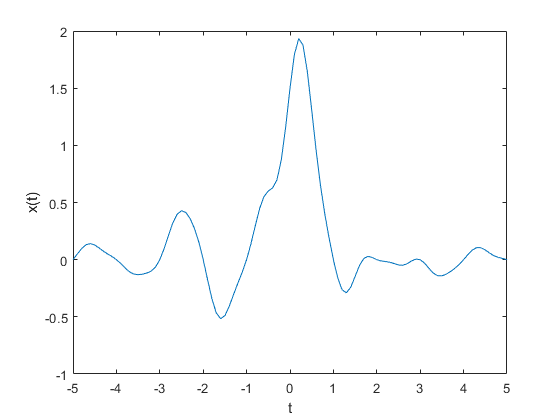
\includegraphics{1.png}
    \caption{Exercise 1}
    \label{fig:1}
\end{figure}
\subsection{Exercise 2}
We start by solving the spectrum for $x(t)$:
\begin{align*}
    x(t) &= [\frac{3}{2} + \frac{3}{10}sin(2\pi t)+sin(\frac{2\pi}{3}t)-sin(\frac{2\pi}{10}t))]sinc(t)\\
     &=  [\frac{3}{2}+\frac{3}{10}\frac{1}{2j}(e^{j2\pi t}-e^{-j2\pi t})+\frac{1}{2j}(e^{j\frac{2\pi}{3} t}-e^{-j\frac{2\pi}{3} t})+\frac{1}{2j}(e^{j\frac{2\pi}{10} t}-e^{-j\frac{2\pi}{10} t}))]\frac{1}{\pi t}\frac{1}{2j}(e^{j\pi t}-e^{-j\pi t})\textit{ (Euler's Formula)}\\
     &= [\frac{3}{2}+\frac{3}{20 j}(e^{j2\pi t}-e^{-j2\pi t})+\frac{1}{2 j}(e^{j\frac{2}{3}\pi t}-e^{-j\frac{2}{3}\pi t})-\frac{1}{2j}(e^{j\frac{1}{5}\pi t}-e^{-j\frac{1}{5}\pi t})]\frac{1}{2j}(e^{j\pi t}-e^{-j\pi t}) \\
     &=  \frac{3}{4j\pi t}(e^{j\pi t}-e^{-j\pi t})-\frac{3}{40\pi t}(e^{j\pi t}-e^{-j\pi t})(e^{j2\pi t}-e^{-j2\pi t})+\frac{1}{4\pi t}(e^{j\pi t}-e^{-j\pi t})(e^{j\frac{2}{3}\pi t}-e^{-j\frac{2}{3}\pi t}) \\
     &+\frac{1}{4\pi t}(e^{j\pi t}-e^{-j\pi t})(e^{j\frac{1}{5}\pi t}-e^{-j\frac{1}{5}\pi t}) \\
     &= \frac{3}{4j\pi t}(e^{j\pi t}-e^{-j\pi t})-\frac{3}{40\pi t}(e^{j\pi t}-e^{-j\pi t}+e^{3j\pi t}-e^{-3j\pi t}))+\frac{1}{4\pi t}(e^{j\pi t}-e^{-j\pi t}+e^{j\frac{5\pi}{3} t}-e^{-j\frac{5\pi}{3} t}) \\
     &+\frac{1}{4\pi t}(e^{j\pi t}-e^{-j\pi t}+e^{j\frac{6\pi}{5} t}-e^{-j\frac{6\pi}{5} t})
  \end{align*}
  
From the last equation, we see that the maximum angular frequency is $w_{max} = 3\pi \text{ rad/s}$ which, after converting, gives us$ f_{max} = 1.5 Hz$. The minimum angular frequency is $w_{min} = \frac{6}{5}\pi \text{ rad/s} \implies f_{min} = 0.6 Hz$. \\
The bandwidth of $x(t)$ is then $f_{max}-f_{min} = 1.5-0.6 = 0.9 Hz$.\\
The sampling theorem states that the sample rate must be atleast two times larger then our max frequency $1.5 Hz$, hence sampling rate must be atleast $3 Hz$. To achieve this rate of samples the time $T_s$ must be $f=\frac{1}{T_s} \implies T_s = \frac{1}{f} = \frac{1}{3}$. \\
 \\
 $\therefore T_s = \frac{1}{3}$s and the bandwidth $ = 0.9 Hz$
%\\
%The sampling theorem states that the sample rate $f_s = 1/T_s$ must be a minimum of $2f_{max}$. Since the maximum frequency is $f_{max} = 2*pi$ 
\subsection{Exercise 3}
With the interval $T_s = \frac{1}{3}$ an almost identical graphical representation of the original signal is shown, see figure \ref{fig:3}.
\begin{figure}
    \centering
    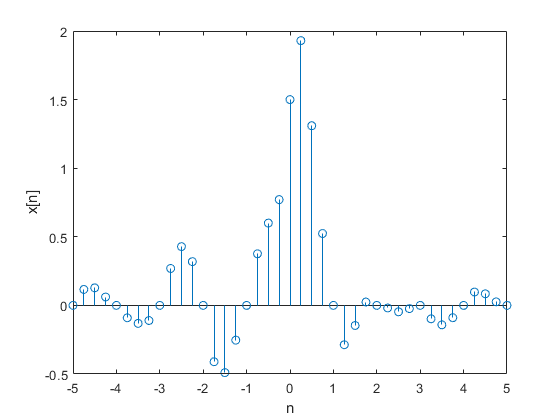
\includegraphics{3.png}
    \caption{Exercise 3}
    \label{fig:3}
\end{figure}

\subsection{Exercise 4}
The sampling theorem specifies a minimum-sampling rate where a properly sampled signal can be reconstructed from the samples. The rate $T_s = \frac{1}{4}$ that we solved in Exercise 2 will then be enough to reconstruct the signal.

\subsection{Exercise 5}
The command $\textit{hold}$ in Matlab helps with drawing these figures you are about to see. By allowing us to draw over a already present plot helps us showcase continuous-time signals by using two instances to plot multiple functions.
We plot equation $a,b,c,d$ in figure \ref{fig:5a},\ref{fig:5b},\ref{fig:5c},\ref{fig:5d}, respectively. We progressivly see a closer representation of $x(t)$ (Orange in figures \ref{fig:5a} - \ref{fig:5d}) from exercise 1.For equation $d$ in figure \ref{fig:5d} we use the value $r = 1000$ which gives an almost exact representation of $x(t)$. \\

\begin{figure}
    \centering
    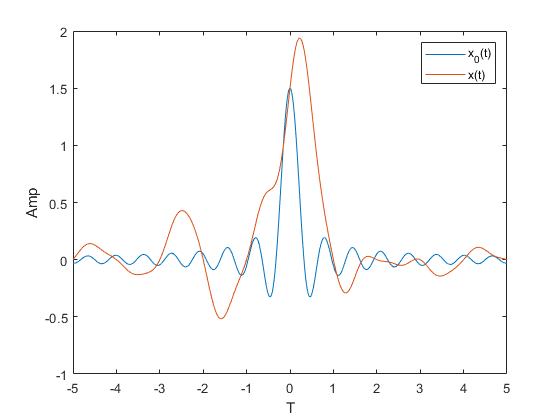
\includegraphics{5a.png}
    \caption{Exercise 5: a}
    \label{fig:5a}
\end{figure}

\begin{figure}
    \centering
    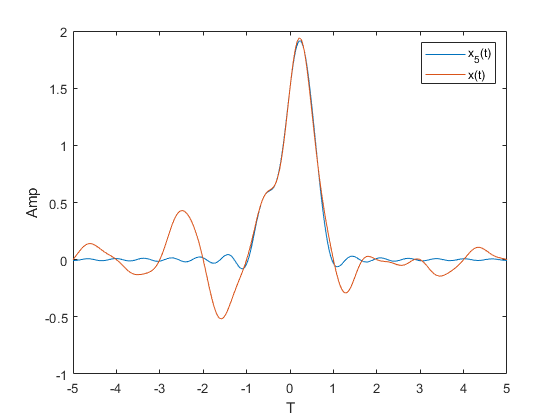
\includegraphics{5b.png}
    \caption{Exercise 5: b}
    \label{fig:5b}
\end{figure}
\begin{figure}
    \centering
    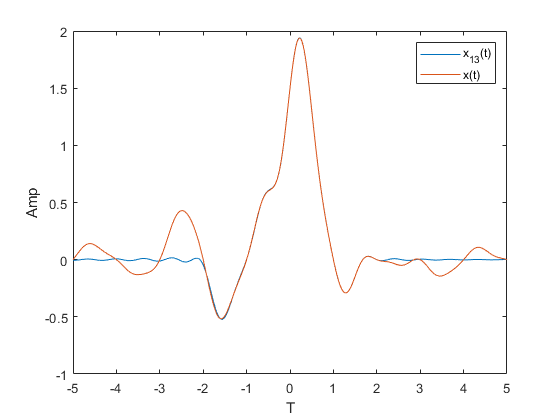
\includegraphics{5c.png}
    \caption{Exercise 5: c}
    \label{fig:5c}
\end{figure}
\begin{figure}
    \centering
    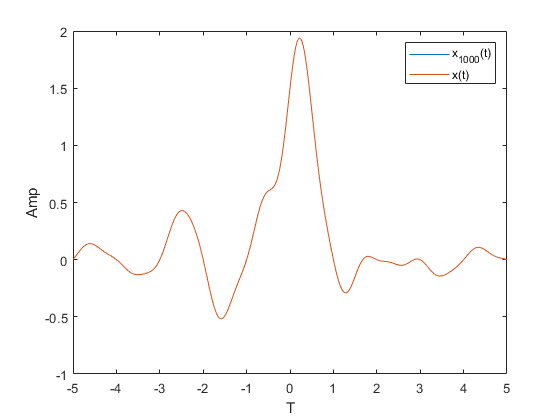
\includegraphics{5d.png}
    \caption{Exercise 5: d}
    \label{fig:5d}
\end{figure}



\end{document}
